\documentclass{article}
\usepackage{amsmath}
\usepackage[UTF8]{ctex}
% 设置页面的环境,a4纸张大小,左右上下边距信息
\usepackage{multirow}
\usepackage[a4paper,left=20mm,right=20mm,top=15mm,bottom=15mm]{geometry}
% 使用indentfirst宏包
\usepackage{indentfirst}
% 设置首行缩进距离
\usepackage{graphicx}
\usepackage{amsthm}
\usepackage{tcolorbox}
%一些奇怪的公式框框!
\newtheorem{mythm}{定理}

\newtcolorbox{mythmbox}{
    arc=0mm,
    colback=white!90!blue,
    colframe=white!90!blue,
    fonttitle=\bfseries,
    title=定理,
    width=.9\linewidth,
    halign title=center
}



%----------------------------------------
\setlength{\parindent}{2em}

\begin{document}
\title{关于阿贝尔规范场与超导统计力学模型对偶的讨论}
\author{刘宇}

\maketitle


\begin{abstract}
    本文主要参考Peskin的文章"Mandelstam-‘t Hooft Duality in Abelian Lattice Models"。
    回顾了对于三维的XY model和三维的零温超导体(英文简称:FZS),以及四维周期性量子电动力学(英文简称:PQED)
    与四维FZS的对偶的推导。表明截然不同的模型的配分函数和关联函数可以通过对偶联系起来。并且可以通过一个模型的性质导出
    另一个模型很多的类似性质。
\end{abstract}

\tableofcontents
\newpage

\section{本文的notation}
本文之中,我们推导考虑的是格点场论。
也就是说,我们认为整个系统是生活在离散的格点上的
因此对于积分我们改成求和;对于空间中的点的位置,我们使用“n”来标记
;而对于空间中每一个点附近其他的点的基矢量,我们使用 $ \hat \mu$来标记。

对于生活在网格空间上的场根据维度不同分为很多不一样的:

首先是生活在格点上的场,我们可以用格点坐标来标定。例如:$\theta_n$

其次对于生活在格点连线上的场,我们可以用格点以及一个方向表示(注意方向正反算两个方向)。例如:$ A_{n,\mu}$

之后对于生活在方格上面的场,我们可以用格电以及两个方向表示。例如:$F_{n,\mu,\nu}$

根据上方的语言我们可以在格点上改写我们熟知的连续的量子场论。值得额外注意的是,对于格点连线和格点方格上面的场其实可以认为是有
方向性的,方向性是由描述他们的方向$\mu$或者$\mu,\nu$决定的。

\section{3-D XY model与3-D FZS对偶}

首先我们讨论两个几乎纯粹的统计力学模型之间的关系。(当然XY model也可以说是一种欧几里德量子场论)。我们的目的是
受到这两个模型之间对偶的推导的启发,用类似的方法推导PQED作为一种欧几里得阿贝尔规范场和FZS作为一种统计力学模型之间的对偶。




\subsection{三维XY model基本介绍}
为保证本文阅读顺畅,我需要先对主要讨论的对象XY model进行介绍。
对于普通的XY model我们写出配分函数是:
\begin{equation}
    Z_{XY} = \int_{\theta}  exp{ ( - \frac{1}{T} (- \sum_{n,\mu} \cos(\theta_{n+ \hat \mu} - \theta_n)) )}
\end{equation}
但本文中讨论XY model需要和动力学的电磁场相耦合的情况。因此引入电磁场后配分函数变为:

\begin{equation}
    Z_{XY} = \int_{\theta}  exp{ ( \frac{1}{T}  \sum_{n,\mu} \cos(\theta_{n+ \hat \mu} - \theta_n - A_{n,\mu})  - \frac{1}{4e^2} \sum_{n,\mu,\nu} F_{n,\mu,\nu}^2 )}
\end{equation}
其中$A_{n,\mu}$表示的是离散的四矢量势,而对应的$F_{n,\mu,\nu}$表示的是离散的电磁场张量,其定义为:
\begin{equation}
    F_{n,\mu,\nu} = (A_{n+\hat \mu,\nu}- A_{n,\nu}) - (A_{n+\hat \nu , \mu} - A_{n, \mu})
\end{equation}
下方图片可以简单的画出这个指的是什么
\begin{figure}[htbp]
    \centering
    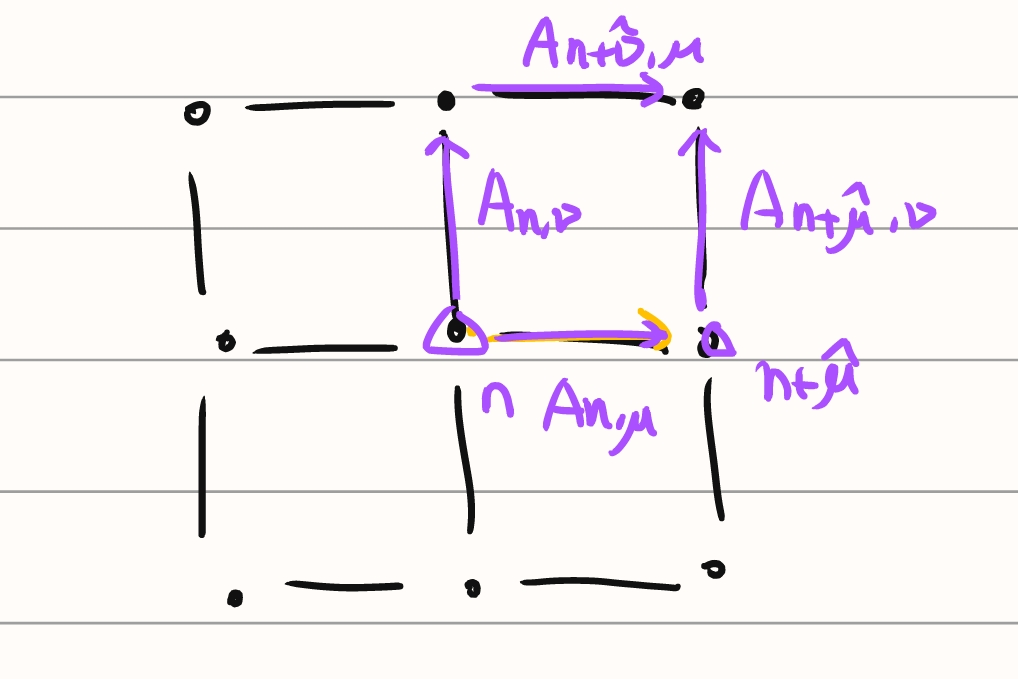
\includegraphics[scale=0.2]{1.jpg}
    \caption[short]{图示格点电磁场张量}
    \label{figure}
\end{figure}

根据已经知道的结论这个模型具有两个相,其相图可以见下方图2。

\begin{figure}[h]
    \centering
    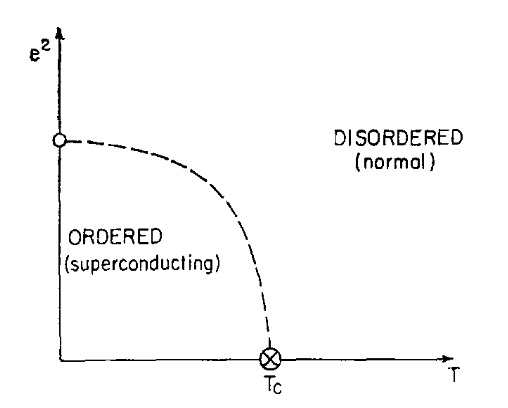
\includegraphics[scale=0.7]{2.png}
    \caption[short]{XY model和电磁场耦合相图}
    \label{figure}
\end{figure}

\subsection{三维格点XY model和三维FZS对偶}
本节之中我们将会证明没有电磁场耦合的三维的XY model和电磁场耦合下的零温超导体的配分函数和关联函数
存在着一一映射。而由于配分函数和关联函数决定着系统的性质,如相变和临界性质。我们可以通过对偶从一个系统的
性质推广到另一个系统的性质。

一个值得注意的事情就是没有电磁场耦合的XY model可以认为是e趋近于0的XY model。因为,e趋近于0的时候
一旦电磁场张量不为0那么该项对于配分函数求和的贡献是无限趋近于0的。因为该项正比于
$exp(- \frac{1}{e^2}(F_{n,\mu,\nu}^2))$这一项趋于0.因此相当于屏蔽了电磁场。

\subsubsection{配分函数对偶}
对于屏蔽电磁场的XY model写出配分函数。
\begin{equation}
    Z_{XY} = \int_{\theta}  exp{ ( \frac{1}{T} \sum_{n,\mu} \cos(\theta_{n+ \hat \mu} - \theta_n)) }
\end{equation}
由于$\cos$函数比较难分析,我们可以保证函数形状类似把cos函数变成很多不同位置的高斯积分的求和。由于在e的指数上,所以都是正数可以进行如此变换,
我们称为Villianization:
\begin{equation}
    exp(\frac{1}{T} \cos(\theta)) \rightarrow  \sum_{m = - \infty}^{\infty} exp(- \frac{1}{2T} (\theta -2 \pi m)^2)
\end{equation}
其中m必然是整数。在此我们对于XY model的配分函数变换为:
\begin{equation}
    Z_{XY} = \prod_n \int_{- \pi}^{\pi} \frac{d \theta_n}{2 \pi} \prod_{n,\mu} \sum_{m_{n,\mu} = -\infty}^{\infty} exp ( - \frac{1}{2T} \sum_{n,\mu} (\theta_{n+ \hat \mu} - \theta_n - 2\pi m_{n,\mu})^2 )
\end{equation}
提示,$m_{n,\mu}$是生活在格点连线上面的场。
这个时候我们发现配分函数在下方变换下不变:
\begin{equation}
    \theta_n \rightarrow \theta_n + 2 \pi N_n \quad m_{n,\mu} \rightarrow m_{n,\mu} + N_{n+ \hat \mu} - N_n
\end{equation}
其中N是整数。
我们的一个目的是希望对于$\theta$的积分是从$- \infty$到$+ \infty$的。我们如果取一些固定的$N_n$那么就可以让$\theta$
从$- \infty$积分到$+ \infty$。我们可以把对于$\theta$的约束转变为对于m的约束。配分函数可以改写为下方两个式子
:

\begin{equation}
    Z_{XY} = \prod_n \int_{- \infty}^{\infty} \frac{d \theta_n}{2 \pi} \prod_{n,\mu} \sum_{m_{n,\mu} = -\infty}^{\infty} exp ( - \frac{1}{2T} \sum_{n,\mu} (\theta_{n+ \hat \mu} - \theta_n - 2\pi m_{n,\mu}) ^2)
\end{equation}
\begin{equation}
    \sum_{\mu} (m_{n+\hat \mu, \mu} - m_{n,\mu}) = 0
\end{equation}

接下来由于配分函数是高斯积分我们可以对高斯积分进行傅立叶变换。我们记:
\begin{equation}
    \theta_{n+ \hat \mu} - \theta_n - 2\pi m_{n,\mu} = \gamma_{n,\mu}
\end{equation}
\begin{equation}
    exp(-\frac{1}{2T} \gamma_{n,\mu}^2) = \int_{- \infty}^{\infty} \frac{d b_{n,\mu}}{2 \pi}  exp{(i b_{n,\mu} \cdot \gamma_{n,\mu}) } \cdot \sqrt[]{2 \pi T} \cdot exp{(- \pi^2 2 T (\frac{b_{n,\mu}}{2 \pi})^2)}
\end{equation}

化简后带入配分函数
\begin{equation}
    Z_{XY} = \prod_n \int_{- \infty}^{\infty} \frac{d \theta_n}{2 \pi} \prod_{n,\mu} \sum_{m_{n,\mu} = -\infty}^{\infty}  \prod_{n,\mu} exp ( - \frac{1}{2T}(\gamma_{n,\mu})^2 )
\end{equation}
代入之后为:
\begin{equation}
    \begin{split}
        Z_{XY} = \prod_n \int_{- \infty}^{\infty} \frac{d \theta_n}{2 \pi} \prod_{n,\mu} \sum_{m_{n,\mu} = -\infty}^{\infty}  \prod_{n,\mu} \int_{- \infty}^{\infty} db_{n,\mu} \sqrt{\frac{T}{2 \pi}} \\
        \times exp\left( -\frac{T}{2} \sum_{n,\mu}b_{n,\mu}^2 + i \sum_{n,\mu} b_{n,\mu} \left( \theta_{n+\hat \mu} - \theta_n - 2 \pi m_{n,\mu} \right) \right)   
    \end{split}
\end{equation}
\begin{equation}
    \sum_{\mu} (m_{n+\hat \mu, \mu} - m_{n,\mu}) = 0
\end{equation}
这个时候我们对于全部的$\theta_n$进行积分可以得到:
\begin{equation}
    \int_{-\infty}^{\infty} \frac{\theta_n}{2 \pi} exp \left( i \theta_n \sum_{\mu} \left( b_{n-\hat \mu,\mu} - b_{n,\mu}\right) \right)  = \delta \left( \sum_{\mu} \left( b_{n-\hat \mu,\mu} - b_{n,\mu}\right)\right) 
\end{equation}
因此我们得到对于配分函数第二约束:
\begin{equation}
    \sum_{\mu} \left( b_{n-\hat \mu,\mu} - b_{n,\mu}\right)= 0
\end{equation}

由于我们在三维的欧几里得空间之中讨论问题。我们可以认为上方的约束条件等价于:
\begin{equation}
    b_{n,\mu} = \sum_{\nu,\sigma} (a_{n-\hat \sigma,\sigma} - a_{n-\hat\nu - \hat \sigma,\sigma})
\end{equation}
值得注意的是,这个条件很强,是由我们讨论的三维欧几里得时空保证的。特别是使用三阶的全反对称算符已经体现了维度。如果在更高维度的时空或者一些具有奇特性质的空间之下并不能保证约束下场一定是式17的形式。


而为了满足约束,
我们用$a_{n,\mu}$场来替代所有的$b_{n,\mu}$ 场。
这个时候我们可以改写配分函数。这里我们使用记号$\int_{a}$指对于所有可能的a configuration的积分;同理$\sum_{m}$指对于所有m的configuration的求和。
具体计算如下:
\begin{equation}
    \begin{split}
        \sum_{n,\mu}\left( \sum_{\nu,\sigma} \epsilon_{\mu,\nu,\sigma}\left( a_{n-\hat \sigma,\sigma} - a_{n-\hat \nu - \hat \sigma,\sigma}\right)   \right)^2 = \\
        \sum_{n,\nu,\sigma}\left[ \left(a_{n+\nu,\sigma}-a_{n,\sigma} \right) - \left( a_{n+\sigma,\nu} - a_{n,\nu} \right)   \right]^2 /2  
    \end{split}
\end{equation}
这个时候我们记:
\begin{equation}
    \begin{split}
        f_{n,\nu,\sigma} =\left( a_{n+\nu,\sigma}-a_{n,\sigma} \right) - \left( a_{n+\sigma,\nu} - a_{n,\nu} \right) \\
        M_{n,\sigma} = \sum_{\mu,\nu} \epsilon_{\sigma,\mu,\nu} \left( m_{n+\hat \nu + \hat \sigma,\mu} - m_{n+\hat \sigma , \mu} \right) 
    \end{split}
\end{equation}
在此我们可以使用f代入配分函数,并且可以使用M代替m。由此配分函数可以变形为:

\begin{equation}
    Z_{XY} = \int_{a} \sum_{m} exp \left( -\frac{T}{4} f_{n,\nu,\sigma}^2 + 2 \pi i \sum_{n,\sigma} a_{n,\sigma} M_{n,\sigma} \right) 
\end{equation}
同时不要忘记,之前对于b的约束已经自然满足但是对于M仍然有约束,见式(9)。对于这个约束可以改写为:
\begin{equation}
    M_{n-\hat \sigma,\sigma} - M_{n,\sigma} = 0
\end{equation}
约束可以改写成$\delta$函数并且代入配分函数。我们有:
\begin{equation}
    \delta \left(  \sum_{\sigma} (M_{n-\hat \sigma,\sigma} - M_{n,\sigma} )\right) = \int_{ - \infty}^{\infty} \frac{ d \theta_n}{2 \pi} exp \left( -i \theta_n \left(\sum_{\sigma} (M_{n-\hat \sigma,\sigma} - M_{n,\sigma} )\right) \right)  
\end{equation}
这里我们引入了一个傅立叶变换的辅助场$\theta$其物理意义尚且不是很明确。
同时我们知道:
\begin{equation}
    1 = \lim_{t \to 0} exp\left[ - \frac{t}{2} \sum_{n,\mu} M_{n,\mu}^2 \right]   
\end{equation}
将22,23两个式子乘上配分函数,我们可以得到下方配分函数:
\begin{equation}
    \begin{split}
        Z_{XY} = \lim_{t \to 0}  \int_{a} \sum_{M} \int_{\theta} exp \left( -\frac{T}{4} f_{n,\nu,\sigma}^2 \right)\\
        exp \left( 2 \pi i \sum_{n,\sigma} a_{n,\sigma} M_{n,\sigma}  -i \theta_n \left(\sum_{\sigma} (M_{n-\hat \sigma,\sigma} - M_{n,\sigma} )\right) - \frac{t}{2} \sum_{n,\mu} M_{n,\mu}^2   \right) 
    \end{split}
\end{equation}
下面对于M进行求和,我们利用恒等式:
\begin{equation}
    \sum_{M = -\infty}^{\infty} e^{i \phi M} e^{-\frac{t}{2}M^2} = \sqrt{\frac{2 \pi}{t}} \sum_{m = -\infty}^{\infty} e^{-(1/2t)(\phi-2\pi m)^2}
\end{equation}
我们可以重新引入辅助场m。并重新定义
$A_{n,\sigma} = 2 \pi a_{n,\sigma}$
接下来我们可以最终改写XY model的配分函数为:
\begin{equation}
   \begin{split}
    Z_{XY} = \lim_{t \to 0}  \int_{A}  \int_{\theta}\sum_{m} exp \left[-\frac{1}{2t} \sum_{n,\sigma} (\theta_{n+ \hat \sigma} - \theta_n - A_{n,\sigma} - 2 \pi m_{n,\sigma})^2 \right]  \\
    \times exp \left[- \frac{T}{\left(2 \pi\right)^2 }  \frac{1}{4} \sum_{n,\nu,\sigma} F_{n,\nu,\sigma}^2 \right]  
   \end{split}
\end{equation}

我们将上方推导的配分函数和之前写出的和电磁场耦合的villainized的XY model相对比:
\begin{equation}
    Z_{XY} = \int_{\theta}  exp{ ( \frac{1}{T}  \sum_{n,\mu} \cos(\theta_{n+ \hat \mu} - \theta_n - A_{n,\mu})  - \frac{1}{4e^2} \sum_{n,\mu,\nu} F_{n,\mu,\nu}^2 )}
\end{equation}

我们会发现正好对应着温度为0,电荷为$2 \pi \sqrt{\frac{1}{T_1}}$的模型。
其中$T_1$代表着原来并没有和电磁场耦合的XY model的温度。由于我们分析温度确定的系统一般使用亥姆霍兹自由能。根据统计力学的公式
\begin{equation}
    F(T,e) = - \log(Z\left(T,e\right) )
\end{equation}
我们可以得到下方的对偶关系:
\begin{equation}
    F(T_1,e_1^2 = 0) = F\left( T_2 = 0, e_2^2 = \frac{\left(2 \pi\right)^2 }{T_1}\right)
\end{equation}
我们可以得出结论认为3-D XY model和3-D FZS的配分函数存在着对偶

\subsubsection{配分函数对偶的讨论}
我们会发现在一个有温度但是没有电磁场耦合的体系对偶于一个零温但是有电磁场耦合的体系。我们已知没有电磁场耦合的3-D XY model存在着
$T_c$温度处的相变。

因此,我们可以推测,3-D FZS在某一个特定的$e_c$处也存在着类似的相变,而且相变相关的参数可以轻易的通过对偶得到。

\subsubsection{关联函数的对偶}
接下来我们计算关联函数,对于没有电磁场耦合的XY model来说spin-spin关联函数是:
\begin{equation}
    \left\langle e^{i \theta_N}e^{- i \theta_{N'}}\right\rangle = \frac{1}{Z_{XY}}  \prod_n \int_{- \pi}^{\pi} \frac{d \theta_n}{2 \pi} e^{i \theta_N}e^{- i \theta_{N'}}   \prod_{n,\mu} \sum_{m_{n,\mu} = -\infty}^{\infty} exp ( - \frac{1}{2T} \sum_{n,\mu} (\theta_{n+ \hat \mu} - \theta_n - 2\pi m_{n,\mu})^2 )
\end{equation}
和对于配分函数的讨论一样,我们对于关联函数进行变形我们可以得到:

\begin{equation}
    \begin{split}
        \left\langle e^{i \theta_N}e^{- i \theta_{N'}}\right\rangle = \frac{1}{Z_{XY}} \prod_n \int_{- \infty}^{\infty} \frac{d \theta_n}{2 \pi} \prod_{n,\mu} \sum_{m_{n,\mu} = -\infty}^{\infty}  \prod_{n,\mu} \int_{- \infty}^{\infty} db_{n,\mu} \sqrt{\frac{T}{2 \pi}} \\
        \times exp\left( -\frac{T}{2} \sum_{n,\mu}b_{n,\mu}^2 + i \sum_{n,\mu} b_{n,\mu} \left( \theta_{n+\hat \mu} - \theta_n - 2 \pi m_{n,\mu} \right) + i\theta_N - i\theta_{N'} \right)   
    \end{split}
\end{equation}

这个时候对于$\theta_n$进行积分,除了$n = N$以及$n = N'$的情况都可以得到之前对于b的约束,而对于这两种特殊情况必须$\pm 1$
因此对于spin-spin关联函数来说对于b的约束应该改为:

\begin{equation}
    \sum_{\mu} \left( b_{n-\hat \mu,\mu} - b_{n,\mu}\right)= \delta_{n,N} - \delta_{n,N'}
\end{equation}

同样的为了保证约束成立我们认为b需要满足一个特殊的形式:
\begin{equation}
    b_{n,\mu} = \sum_{\nu,\sigma} (a_{n-\hat \sigma,\sigma} - a_{n-\hat\nu - \hat \sigma,\sigma})  + L_{n,\mu}
\end{equation}
其中$L_{n,\mu}$是一个格点连线上的场,对于某一条特定的N到N'格点的连线上,$L_{n,\mu}$取值为1,其他连线上取值皆为0.
我们可以直观的认为$L_{n,\mu}$可以写成N到N'点的一条线。如下图3所示。

\begin{figure}[h]
    \centering
    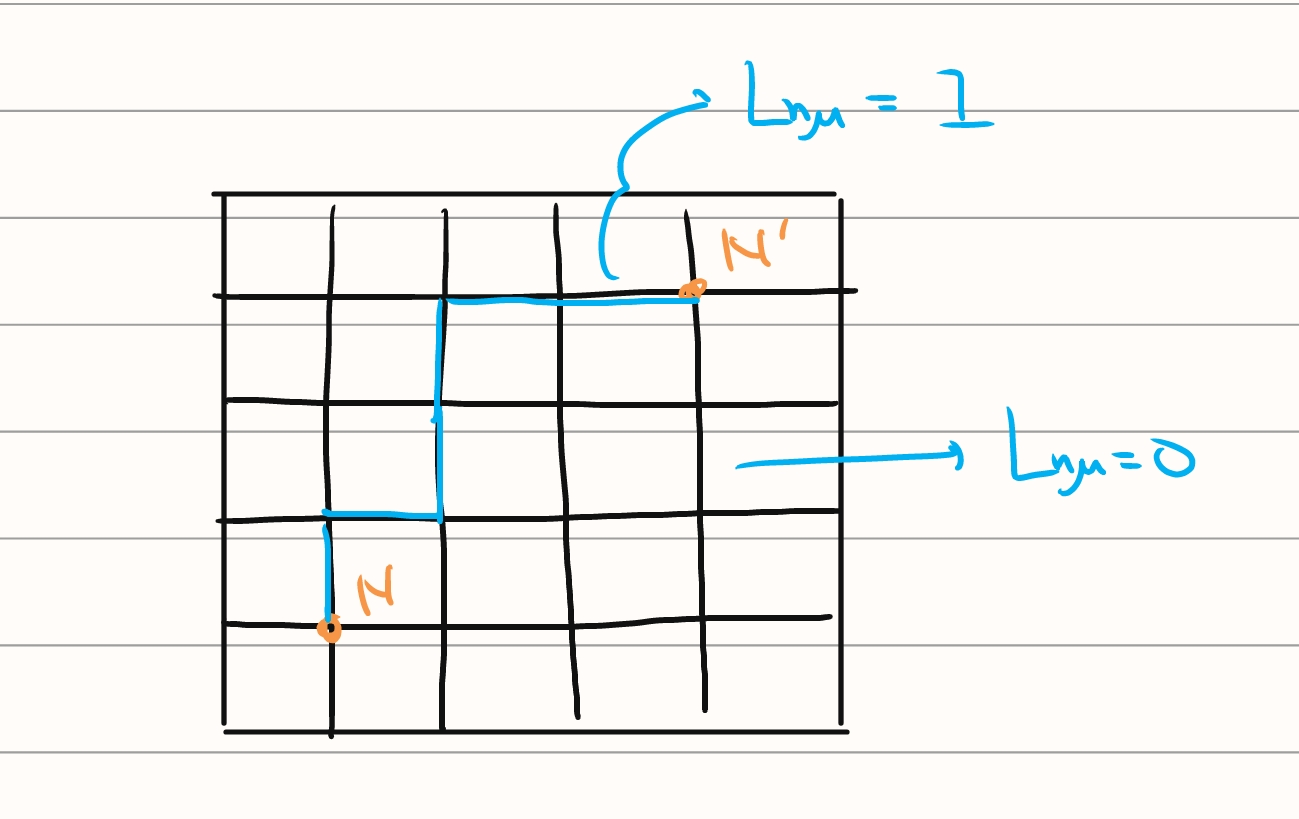
\includegraphics[scale=0.2]{3.jpg}
    \caption[short]{图示$L_{n,\mu}$取值}
    \label{figure}
\end{figure}
对于端点的线上的点,由于每个格点相邻有两条格点连线不为0,因此在对于$b_{n-\hat \mu,\mu}-b_{n,\mu}$的求和下会得到0,而仅有端点处求和为1。
正好满足b的约束条件的delta函数。
积分$\theta_n$之后的关联函数可以写成:

\begin{equation}
    \left\langle e^{i \theta_N}e^{- i \theta_{N'}}\right\rangle  = \frac{1}{Z_{XY}} \int_a \sum_{m_{\mu,\nu}} exp \left[-\frac{T}{2} \sum b_{n,\mu}^2 - 2 \pi i \sum b_{n,\mu} m_{n,\mu} \right] 
\end{equation}
代入b的定义之后我们会发现由于L和m都是整数取值,其中$L_{n,\mu} \cdot m_{n,\mu}$项都可以消去,因为:
\begin{equation}
    exp\left[ 2 \pi i \sum L_{n,\mu} m_{n,\mu}\right] = 1
\end{equation}
同时考察$b^2$项,类似于之前的计算我们有:
\begin{equation}
    \begin{split}
        \sum_{n,\mu} \left(b_{n,\mu}\right)^2  = \sum_{n,\nu,\sigma} \frac{1}{2}\left(f_{n,\nu,\sigma}\right)^2 + a\sum_{n,\mu,\nu,\sigma} \epsilon_{\mu\nu\sigma} (a_{n-\sigma,\sigma}- a_{n-\nu-\sigma,\sigma})L_{n,\mu} + \sum_{n,\mu} L_{n,\mu}^2\\
         = \sum_{n,\nu,\sigma} \frac{1}{2}\left(f_{n,\nu,\sigma}\right)^2 +\sum_{n,\nu,\sigma} (f_{n,\nu,\sigma})\sum_{mu}\epsilon_{\mu\nu\sigma}L_{n+\nu+\sigma,\mu}+\sum_{n,\mu} L_{n,\mu}^2\\
         = \sum_{n,\nu,\sigma} \frac{1}{2}\left(f_{n,\nu,\sigma}+\sum_{\mu} \epsilon_{\mu\nu\sigma}L_{n+\nu+\sigma,\mu}\right)^2 
    \end{split}
\end{equation}
其中第二步进行了换元$n \to n+\nu+\sigma$经过这样的变形我们可以重新定义:
\begin{equation}
    \hat f_{n,\nu,\sigma} = f_{n,\nu,\sigma}+\sum_{\mu} \epsilon_{\mu\nu\sigma}L_{n+\nu+\sigma,\mu}
\end{equation}
后续推导过程和配分函数完全相同因此省略,最后我们可以得到关联函数为:

\begin{equation}
    \begin{split}
        \left\langle e^{i \theta_N}e^{- i \theta_{N'}}\right\rangle = \frac{1}{Z_{XY}} \lim_{t \to 0}  \int_{A}  \int_{\theta}\sum_{m} exp \left[-\frac{1}{2t} \sum_{n,\sigma} (\theta_{n+ \hat \sigma} - \theta_n - A_{n,\sigma} - 2 \pi m_{n,\sigma})^2 \right]  \\
     \times exp \left[- \frac{T}{\left(2 \pi\right)^2 }  \frac{1}{4} \sum_{n,\nu,\sigma} \hat F_{n,\nu,\sigma}^2 \right]  
    \end{split}
 \end{equation}

其中:
\begin{equation}
    \hat F_{n,\nu,\sigma}^2 = F_{n,\nu,\sigma}+ 2 \pi \sum_{\mu} \epsilon_{\mu\nu\sigma}L_{n+\nu+\sigma,\mu}
\end{equation}
这个时候我们会发现得到了一个电磁场张量发生一定变化的零温超导体系统。而其变化正好等价于存在一个狄拉克弦(或者认为是某种规范下的磁单极子在超导体之中存在)。
而根据:
\begin{equation}
    F = -\log(Z)
\end{equation}
我们有:
\begin{equation}
    \left\langle e^{i \theta_N}e^{- i \theta_{N'}} \right\rangle _{XY} = exp\left(-\left(F_{dirac_string} - F_{FZS}\right) \right) = exp\left(- \Delta F(e_2, N-N')\right)_{(FZS)} 
\end{equation}

\subsubsection{关联函数对偶的讨论}
我们会发现可以通过求解一个没有电磁场耦合的XY model的spin-spin关联函数得到磁单极子存在导致的FZS的
亥姆霍兹自由能的增加量。也就是相当于磁单极子的能量。

而更有意义的是,由于我们知道XY model存在着相变。那么,我们会认为在一个特殊的$e_c$上下零温超导体存在着相变,使得超导体之中存在两个反号的磁单极子的时候
能量按照不同方式提升。

当$T < T_c$也就是$e>e_c$时候:
\begin{equation}
    \left\langle e^{i \theta_N}e^{- i \theta_{N'}} \right\rangle _{XY} = exp\left(- \Delta F(e_2, N-N')\right)_{(FZS)}  = |\Phi_0|^2 \times \left(1-\frac{1}{\rho_s(T)}\int \frac{d^3 q}{(2\pi)^3}\frac{e^{-q \cdot n}}{q^2} +\dots \right) 
\end{equation}
\begin{equation}
    \Delta F(e_2, N-N')_{(FZS)}= -2 \log(|\Phi_0(T)|) - \frac{1}{\rho_s(T)}\frac{1}{4 \pi |N-N'|}
\end{equation}
根据第二项我们会发现磁单极子相互作用为库伦相互作用。也就是正常的电磁场态,因此这种情况下系统其实并不是超导体。


当$T > T_c$也就是$e<e_c$时候:
\begin{equation}
    \left\langle e^{i \theta_N}e^{- i \theta_{N'}} \right\rangle _{XY} = exp\left(- \Delta F(e_2, N-N')\right)_{(FZS)}  = e^{- \frac{|N-N'|}{\xi(T)}}
\end{equation}
\begin{equation}
    \Delta F(e_2, N-N')_{(FZS)}= C \times |N-N'|
\end{equation}
这个时候,磁单极子的亥姆霍斯自由能正好满足超导体的要求。

总而言之我们会发现,在$e_c$处发生了超导相变。


\section{4-D PQED 与4-D FZS的对偶}
上方我们讨论了两个统计力学模型之间的对偶(当然电磁场耦合的XY model也可以认为是欧几里得量子场论)。但是其中推导的
思路可以推广到四维。而这个时候我们会研究一个阿贝尔规范场体系,也就是PQED。我将先对于这个模型进行介绍然后推导其对偶关系。

\subsection{配分函数对偶}
在这里我们定义PQED的配分函数。PQED是一种量子电动力学,但是这里我们认为
$A_{n,\mu}$不再是电动力学的基本的变量,取而代之的是$U_{n,\mu} = exp\left[ -i A_{n,\mu}\right] $
。因此,我么可以看出A的取值是有$2 \pi$周期性的。

接下来我们写出PQED的配分函数(或者其实就是欧几里得路径积分的配分函数):
\begin{equation}
    Z = \int_A exp\left[ - \frac{1}{4 g^2} \sum_{\mu,\nu} \left(U_{n,\mu}U_{n+\mu,\nu}U_{n+\nu,\mu}^{\dagger} U_{n,\nu}^{\dagger} +c.c.\right)   \right] 
\end{equation}
代入U和F的定义我们不难发现配分函数可以改写成:
\begin{equation}
    Z = \int_A exp\left[ \frac{1}{g^2} \sum_{\mu,\nu} \cos(F_{n,\mu,\nu})  \right] 
\end{equation}
我们不难发现这个配分函数和XY model很像,一个最大区别是基本的场变成了生活在格点连线上的。因此,为了类比XY model我们考虑的是四维的情况。
接下来我们和之前一样把配分函数villainization变换为:
\begin{equation}
    Z = \prod_{n,\nu}\int_{- \pi}^{\pi}\frac{d A_{n,\mu}}{2 \pi} \prod_{n,\mu,\nu} \sum_{m_{n,\mu,\nu} = -\infty}^{\infty} exp\left[ - \frac{1}{2g^2}\sum_{n,\mu<\nu}\left(F_{n,\mu,\nu} - 2 \pi m_{n,\mu,\nu}\right)^2 \right] 
\end{equation}
同样的我们试图通过对于m进行约束把对于A的积分拓展到整个实轴上面。同时,进行傅立叶变换产生辅助场g。由于这些计算和三位的情况完全一样所以在此省略细节。
但是需要特别注意的是,对于A进行积分得到对于傅立叶变换后的辅助场g的约束写为:
\begin{equation}
    \sum_{\nu} \left(g_{n,\mu,\nu} - g_{n-\nu,\mu,\nu}\right) = 0 
\end{equation}
对于四维的情况之下我们发现满足上面的g需要满足下方的关系:
\begin{equation}
    g_{n,\mu,\nu} = \sum_{\lambda,\sigma}\epsilon_{\mu\nu\lambda\sigma} f_{n-\lambda-\sigma,\lambda,\sigma}
\end{equation}
同时类比之前的推导我们定义:
\begin{equation}
    M_{n,\sigma} = \frac{1}{2}\sum_{\mu,\nu,\lambda} \epsilon_{\sigma\lambda\mu\nu}\left(m_{n+\sigma+\lambda,\mu,\nu}- m_{n+\sigma,\mu,\nu}\right) 
\end{equation}
我们代入配分函数之后吗,再利用最开始m的约束变成辅助场$\theta$,再进行类似之前推导的恒等变换(引入m场!)可以得到:
\begin{equation}
    \begin{split}
        Z = \lim_{t \to 0} \int_A \int_{\theta} \sum_{m} exp\left[- \frac{1}{2t} \sum_{n,\sigma} \left(\theta_{n+\sigma} -\theta_n - A_{n,\sigma} - 2 \pi m_{n,\sigma}  \right)^2   \right] \\
        \times exp\left[- \frac{g^2}{(2\pi)^2} \frac{1}{4} \sum_{n,\nu,\sigma} F_{n,\nu,\sigma}^2   \right] 
    \end{split}
\end{equation}
很快我们会发现PQED对偶于一个四维的FZS。

相应的根据对偶我们可以推测PQED类似于FZS存在着和耦合常数$g$相关的相变。

\subsection{关联函数对偶}
对于关联函数,其实可以理解为系统的一个描述“序”的可观测量的对偶。
而对于四维的PQED,根据之前Wilson的工作,我们可以使用Wilson Loop作为客观测量:
\begin{equation}
    \left\langle \prod_{\{ n,\mu \} \in P} e^{-i A_{n,\mu}} \right\rangle 
\end{equation}
其中P是一个格点空间上的loop。计算wilson loop的期望为:
\begin{equation}
    \begin{split}
        \left\langle \prod_{\{ n,\mu \} \in P} e^{-i A_{n,\mu}} \right\rangle  = \frac{1}{Z} \prod_{n,\nu}\int_{- \pi}^{\pi}\frac{d A_{n,\mu}}{2 \pi} \left(\prod_{\{ n,\mu \} \in P} e^{-i A_{n,\mu}} \right) \\
        \prod_{n,\mu,\nu} \sum_{m_{n,\mu,\nu} = -\infty}^{\infty} exp\left[ - \frac{1}{2g^2}\sum_{n,\mu<\nu}\left(F_{n,\mu,\nu} - 2 \pi m_{n,\mu,\nu}\right)^2 \right] 
    \end{split}
\end{equation}
这时候和之前一样我们利用对m的约束把对A的积分拓展到整个实轴,并且引入傅立叶变换(和之前记号一样我们记辅助场为g)后对A做积分。
这个时候会类似的得到g的约束条件:
\begin{equation}
    \left( \sum_{\nu} g_{n,\mu,\nu} - g_{n- \nu,\mu,\nu} \right)  = - \sum_{\left\{n',\mu'\right\} \in P }\delta_{(n,\mu),(n',\mu')}
\end{equation}
这个时候类比之前XY model的spin-spin 关联函数计算的情况,
我们可以引入$L_{n,\mu,\nu}$认为:
\begin{equation}
    g_{n,\mu,\nu} = \sum_{\lambda,\sigma}\epsilon_{\mu\nu\lambda\sigma} f_{n-\lambda-\sigma,\lambda,\sigma} + L_{n,\mu,\nu}
\end{equation}
而其中L的定义就是在P这个wilson loop围绕成平面内取值为1其他地方取值为0。可以见下方图4所示。
\begin{figure}[h]
    \centering
    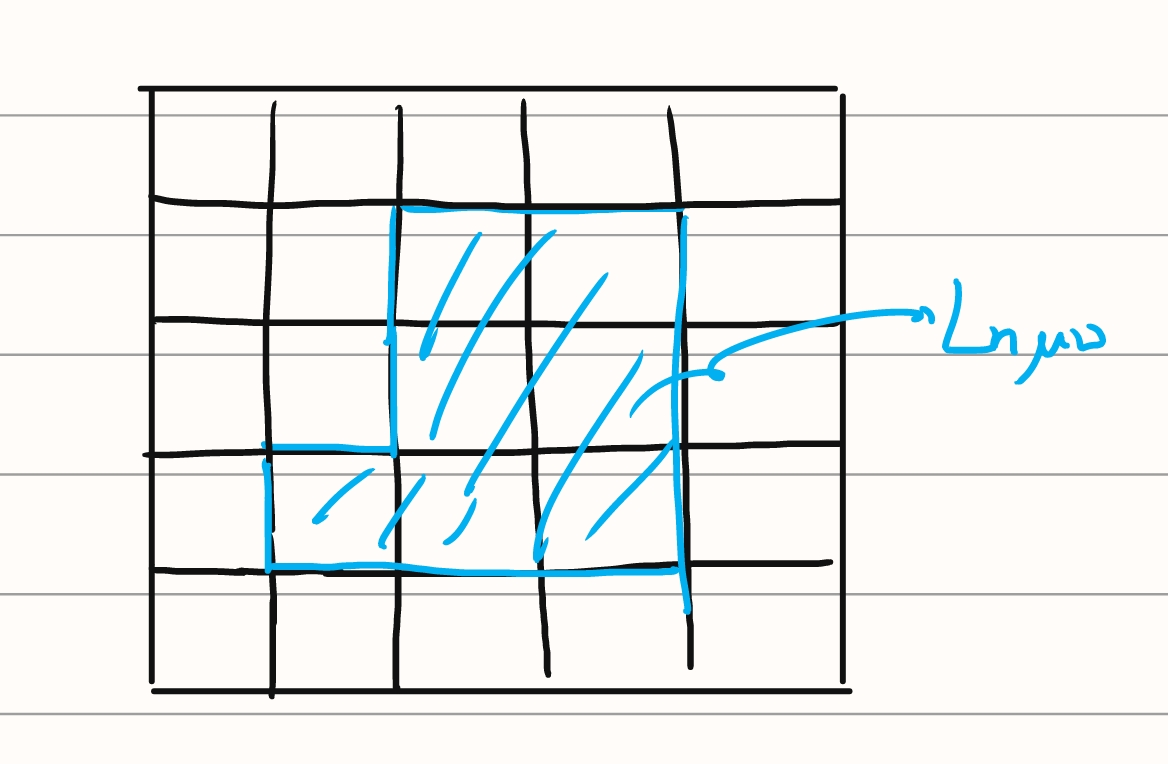
\includegraphics[scale=0.2]{4.jpg}
    \caption[short]{图示$L_{n,\mu,\nu}$取值}
    \label{figure}
\end{figure}
类比三维XY model的情况我们继续变换。可以得到:
\begin{equation}
    \begin{split}
        \left\langle \prod_{\{ n,\mu \} \in P} e^{-i A_{n,\mu}} \right\rangle   = \frac{1}{Z} \lim_{t \to 0} \int_A \int_{theta} \sum_{m} exp \left[ - \frac{1}{2t} \sum_{n,\sigma} \left( \theta_{n+\sigma} - \theta_n - A_{n,\sigma} - 2 \pi m_{n,\sigma} \right)^2  \right] \\
        \times exp\left[ - \frac{g^2}{(2\pi)^2} \frac{1}{4} \sum_{n,\nu,\mu} \hat F_{n,\nu,\sigma}^2 \right] 
    \end{split}
\end{equation}
其中重新定义的$\hat F$是:
\begin{equation}
    \hat F_{n,\nu,\sigma} = \left(F_{n,\nu,\sigma}+ \frac{1}{2} \sum_{\mu,\rho} \epsilon_{\nu\sigma\mu\rho} L_{n+\nu+\sigma,\mu,\rho}\right) 
\end{equation}
最终我们可以认为存在对偶。也即是PQED里面的可观测量wilson loop的期望对偶于FZS之中一个沿着P路径运动的磁流。


\section{总结}
综上我们推导了三维的XY model与FZS的对偶以及四维PQED与FZS的对偶。
我们认识到相差很多的量子场论或者统计力学系统其实有着很深层的联系,而且这样的联系会
定性和定量的帮助我们探索很多模型的性质。





\end{document}